\chapter{Landasan Teori}
\label{chap:pendahuluan}

\section{Mesin Navigasi KIRI}
\label{sec:mesin_navigasi_kiri}

KIRI memiliki mesin navigasi yang dibangun pada bahasa Java. Mesin ini bertugas
untuk menerima masukan berupa koordinat titik asal dan tujuan, kemudian
menemukan angkot-angkot yang harus dinaiki untuk menuju titik tujuan dari
titik asal. Karena alasan kerahasiaan, pembahasan mengenai mesin navigasi
KIRI tidak mengacu pada referensi publik, melainkan dari survei terhadap
kode sumber internal KIRI.

\begin{figure}
\centering
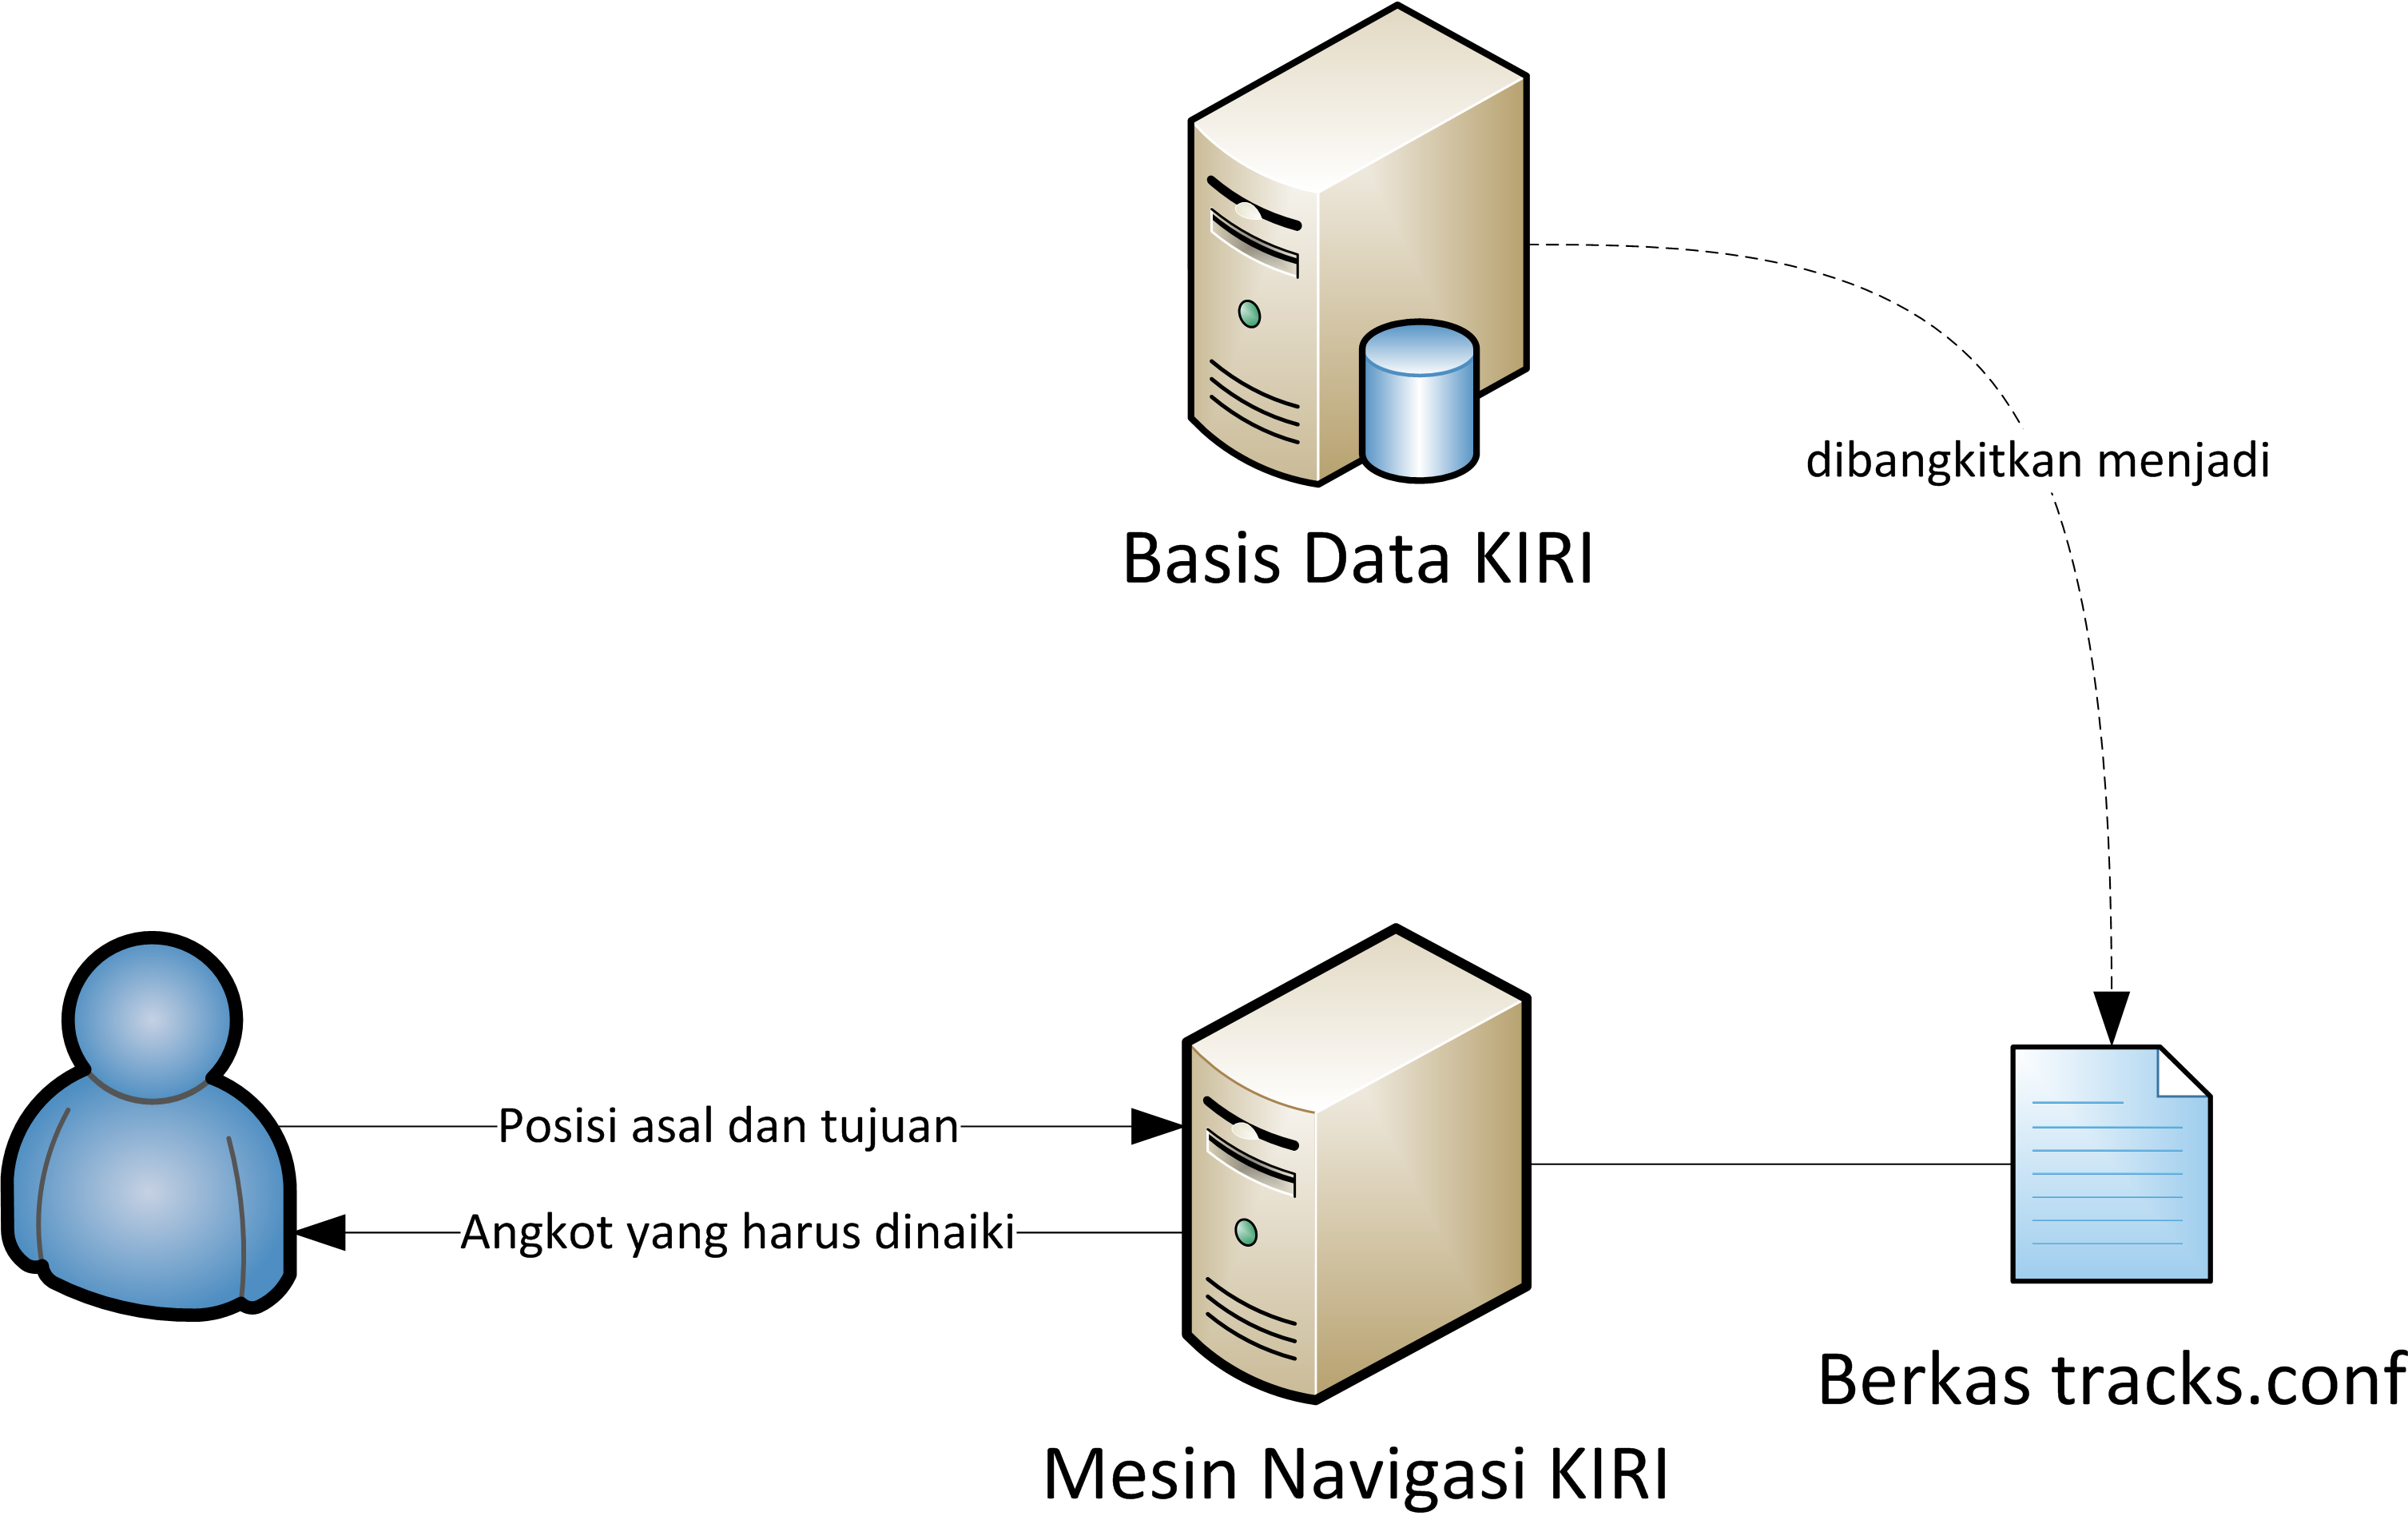
\includegraphics[scale=1]{Gambar/2_arsitektur_saat_ini}
\caption{Arsitektur Saat Ini} 
\label{fig:2_arsitektur_saat_ini}
\end{figure}

Seperti dapat dilihat pada gambar \ref{fig:2_arsitektur_saat_ini}, elemen
arsitektur yang mendukung navigasi KIRI dibagi menjadi tiga, yaitu:
\begin{itemize}
	\item \textbf{Basis Data KIRI} menyimpan informasi rute 33 trayek angkot,
		yang masing-masing mencakup identifikasi trayek (\verb/trackId/ dan
		\verb/trackTypeId/), nama trayek (\verb/trackName/), daftar koordinat
		yang dilewati (\verb/geodata/), informasi pulang-pergi
		(\verb/pathloop/), catatan internal (\verb/internalInfo/), prioritas
		untuk dipilih (\verb/penalty/), informasi naik/turun penumpang
		(\verb/transferNodes/), dan parameter ekstra untuk pembelian
		tiket (\verb/extraParameters/).
	\item \textbf{Berkas tracks.conf} adalah hasil ekstraksi dari basis data
		KIRI, yang menyimpan informasi penting saja yang dibutuhkan oleh algoritma
		mesin navigasi KIRI, yakni: \verb/trackId/, \verb/trackTypeId/,
		\verb/penalty/, \verb/geodata/, \verb/pathloop/, dan
		\verb/transferNodes/.
	\item \textbf{Mesin Navigasi KIRI} adalah program yang bertugas mengolah
		data yang ada pada berkas tracks.conf, sehingga dapat menjawab
		pertanyaan navigasi dari titik asal ke titik tujuan. Karena alasan
		historis, mesin navigasi tidak membaca data langsung dari basis data,
		melainkan dari berkas tracks.conf.
\end{itemize}

\subsection{Basis Data KIRI}
Basis data KIRI disimpan dalam sistem manajemen basis data MySQL. Salah satu
dari tabel yang digunakan adalah tabel \verb/tracks/, yang menyimpan informasi
rute trayek. Struktur dari tabel ini dijelaskan pada tabel
\ref{tab:2_struktur_tabel_tracks}.

\begin{table}
	\caption{Struktur Tabel tracks}
	\label{tab:2_struktur_tabel_tracks}
	\begin{tabular}{|p{3cm}|p{2.5cm}|p{9.5cm}|}
		\hline
		Nama kolom & Tipe & Keterangan \\
		\hline
		trackId & varchar(32) & Kode trayek angkot (misal: "sthallciumbuleuitlurus").
			Menjadi PRIMARY KEY tabel bersama trackTypeId. \\
		trackTypeId & varchar(32) & Kode tipe trayek (untuk angkot bandung,
			selalu berisi "bdo\_angkot"). Menjadi PRIMARY KEY bersama trackId. \\
		trackName & varchar(32) & Nama trayek yang dapat dibaca secara umum
			(misal: "St. Hall - Ciumbuleuit (lurus)"). \\
		internalInfo & varchar(1024) & Informasi internal yang dapat
			ditambahkan dan tidak akan ditampilkan pada hasil pencarian. \\
		geodata & linestring & Daftar koordinat dari rute trayek ini. \\
		pathloop & tinyint(1) & Menandakan apakah trayek ini adalah trayek
			pulang pergi atau satu arah. \\
		penalty & decimal(4,2) & Bobot dari trayek ini. Semakin besar nilainya,
			semakin kecil kemungkinan akan muncul pada hasil navigasi. \\
		transferNodes & varchar(1024) & Daftar indeks titik di mana penumpang
			dapat turun maupun naik, dipisahkan dengan koma. Untuk angkot
			Bandung, penumpang dapat turun dan naik di semua titik. \\
		extraParameters & varchar(256) & Informasi yang ditambahkan saat
		melakukan pembelian tiket (tidak terkait dengan penelitian ini). \\
		\hline
	\end{tabular}
\end{table}

\subsection{Berkas tracks.conf}
Karena alasan historis\footnote{Pada awalnya mesin navigasi KIRI dibangun
menggunakan bahasa C++, sehingga menyulitkan dalam mengakses basis data MySQL},
mesin navigasi KIRI tidak mengakses langsung ke basis data MySQL, melainkan
membaca sebuah berkas yang bernama \verb/tracks.conf/.

Berkas \verb/tracks.conf/ ini merupakan sebuah berkas teks yang menyimpan basis
data trayek yang telah dibersihkan untuk dapat dibaca dengan mudah, satu
\textit{record} per baris. Setiap baris berisi 6 \textit{field} yang dipisahkan
dengan \textit{tab} (\verb/\t/). Penjelasan dari keenam \textit{field} tersebut
dapat dilihat pada tabel \ref{tab:2_struktur_tracks_conf}.

\begin{table}
	\caption{Struktur berkas tracks.conf}
	\label{tab:2_struktur_tracks_conf}
	\begin{tabular}{|p{0.5cm}|p{3.5cm}|p{11cm}|}
		\hline
		No. & Nama \textit{field} & Keterangan \\
		\hline
		1. & trackTypeId.trackId & Berisi \verb/trackTypeId/ dan \verb/trackId/
			dipisahkan dengan titik. \\
		2. & penalty & Berisi nilai \verb/penalty/. \\
		3. & numberOfNodes & Berisi jumlah \textit{node} (titik) dari rute
			trayek ini. \\
		4. & nodes & Berisi daftar koordinat \textit{node} dari rute trayek
			ini dipisahkan dengan \textit{tab}. Setiap koordinat node terdiri
			dari \textit{latitude} dan \textit{longitude} yang dipisahkan
			dengan spasi. \\
		5. & pathLoop & Berisi nilai \verb/pathloop/ yang menunjukkan apakah
			rute ini merupakan rute pulang pergi atau searah. \\
		6. & transferNodes & Berisi nilai \verb/transferNodes/ yang menunjukkan
			titik-titik di mana penumpang diperbolehkan untuk naik / turun. \\
		\hline
	\end{tabular}
\end{table}

\subsection{Mesin Navigasi KIRI}

Mesin navigasi KIRI merupakan sebuah program yang mendengarkan dan menjawab
permintaan navigasi dalam bentuk \textit{HTTP request} di \textit{port} 8000.
Program ini dibangun di atas bahasa Java, yang terdiri dari beberapa kelas yang
ditunjukkan pada gambar \ref{fig:2_diagram_kelas_sistem_kini}.

\begin{figure}
\centering
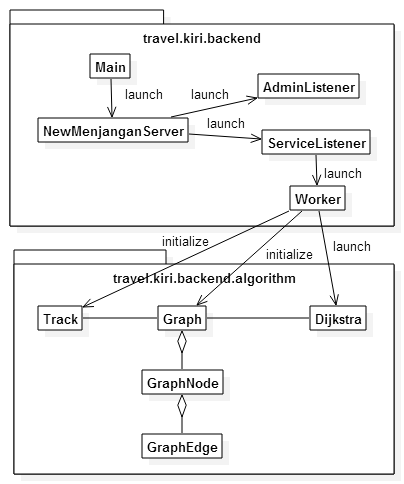
\includegraphics[scale=0.5]{Gambar/2_diagram_kelas_sistem_kini}
\caption{Diagram Kelas Sistem Kini} 
\label{fig:2_diagram_kelas_sistem_kini}
\end{figure}

Penjelasan untuk setiap kelas dapat dilihat pada tabel
\ref{tab:2_penjelasan_kelas_kelas_sistem_kini}.

\begin{table}
	\caption{Penjelasan Kelas-Kelas Sistem Kini}
	\label{tab:2_penjelasan_kelas_kelas_sistem_kini}
	\begin{tabular}{|p{4cm}|p{11cm}|}
		\hline
		Kelas & Keterangan \\
		\hline
		Main & Kelas yang berfungsi sebagai antarmuka program, untuk dijalankan
			dari \textit{console}. \\
		NewMenjanganServer & Kelas yang bertugas menjalankan program sebagai
			server, yakni menyiapkan servis-servis untuk dijalankan. \\
		AdminListener & Kelas yang berfungsi untuk mendengarkan dan merespon
			perintah administrasi, seperti \textit{ping}, \textit{shutdown},
			dll. \\
		ServiceListener & Kelas yang berfungsi untuk mendengarkan dan merespon
			permintaan untuk navigasi. Servis ini menerima masukan berupa
			koordinat asal dan tujuan, dan mengembalikan rute angkot yang harus
			dinaiki. \\
		Worker & Kelas ini berfungsi untuk melakukan pekerjaan yang telah
			diterima oleh ServiceListener. Selain itu, di awal kelas ini juga
			menyiapkan bahan-bahan yang diperlukan untuk melakukan perhitungan
			rute, yakni mengkonversi data trayek ke dalam bentuk graf. \\
		Track & Kelas ini berfungsi untuk menyimpan informasi sebuah trayek
			angkot beserta rutenya. \\
		Graph & Kelas ini merepresentasikan sebuah graf. \\
		GraphNode & Kelas ini merepresentasikan setiap \textit{node} yang
			dimiliki oleh graf. \\
		GraphEdge & Kelas ini merepresentasikan sebuah \textit{edge} dari
			GraphNode. \\
		Dijkstra & Kelas ini merepresentasikan algoritma \textit{Dijkstra's
			shortest path}\cite{Cormen:2001}, untuk digunakan dalam pencarian
			rute. \\
		\hline
	\end{tabular}
\end{table}

\section{Protokol angkot.web.id}
\label{sec:mesin_navigasi_kiri}
Berdasarkan kode sumber angkot.web.id \cite{angkotwebid}, situs angkot.web.id
memanfaatkan \textit{HTTP request} \cite{rfc7231} untuk menerima
perintah-perintah dan mengembalikan respon berupa data dalam sintaks JSON
\cite{rfc7159}. Beberapa dari perintah tersebut dijelaskan pada subbab-subbab
berikut.

\subsection{Transportation List}
Perintah ini digunakan untuk mendapatkan daftar semua daftar transportasi umum,
dan dapat diakses pada dengan melakukan \textit{HTTP request GET}
pada path \verb|/route/transportation-list.json|, tanpa parameter apapun. Adapun
kembalian dari perintah ini adalah:

\begin{itemize}
	\item \verb/status/: Status kembalian dari perintah yang dikirimkan
	\item \verb/provinces/: \textit{Array} provinsi yang terdaftar, masing-
		masing elemen merupakan \textit{array} lain yang berisi:
		\begin{itemize}
			\item Kode provinsi
			\item Nama provinsi
		\end{itemize}
	\item \verb/transportations/: \textit{Array} provinsi yang terdaftar,
		masing-masing berisi:
		\begin{itemize}
			\item \verb/hasroute/: Menyatakan apakah trayek ini memiliki data
				rute
			\item \verb/company/: Perusahaan pengelola trayek ini
			\item \verb/id/: Indeks trayek ini dalam basis data
			\item \verb/origin/: Awal rute trayek
			\item \verb/destination/: Akhir rute trayek
			\item \verb/province/: Provinsi tempat trayek ini beroperasi
			\item \verb/city/: Kota tempat trayek ini beroperasi
			\item \verb/number/: Nomer trayek
			\item \verb/created/: \textit{UNIX time} trayek ini dibuat
			\item \verb/updated/: \textit{UNIX time} trayek ini terakhir diperbaharui
		\end{itemize}
\end{itemize}

Contoh kembalian dari perintah transportation list dapat dilihat pada kode
di bawah ini:

\begin{lstlisting}
{
	"status": "ok",
	"provinces": [
		[
			"ID-AC",
			"Aceh"
		],
		...
	],
	"transportations": [
		{
			"hasRoute": true,
			"company": "KWK",
			"id": 21,
			"origin": null,
			"destination": null,
			"province": "ID-JK",
			"city": "Jakarta",
			"number": "S15A",
			"created": "1379952348",
			"updated": "1379952379"
		},
		...
	]
}
\end{lstlisting}

\subsection{Transportation Detail}
Perintah ini digunakan untuk mendapatkan detail dari sebuah trayek transportasi,
dan diakses dengan melakukan \textit{HTTP request GET} pada path
\verb|/route/transportation/nnn.json| (di mana \textit{nnn} adalah nomer kode
trayek dalam basis data). Adapun kembalian dari perintah ini adalah:

\begin{itemize}
	\item \verb/id/: Nomer kode trayek.
	\item \verb/geojson/: Data rute dan atributnya dalam format
		GeoJSON\cite{geojson}, terdiri dari:
		\begin{itemize}
			\item \verb/type/: Tipe GeoJSON yang digunakan
			\item \verb/properties/: Properti-properti data GeoJSON, terdiri dari:
				\begin{itemize}
					\item \verb/number/: Nomer trayek
					\item \verb/accept/: \textit{tidak diketahui}
					\item \verb/company/: Perusahaan pengelola trayek ini
					\item \verb/destination/: Akhir rute trayek
					\item \verb/province/: Provisi tempat trayek ini beroperasi
					\item \verb/origin/: Awal rute trayek
					\item \verb/city/: Kote tempat trayek ini beroperasi
				\end{itemize}
			\item \verb/properties/: Data geometri rute trayek ini, mengikuti
				standar GeoJSON untuk tipe data \verb/MultiLineString/.
		\end{itemize}
	\item \verb/created/: \textit{UNIX time} trayek ini dibuat
	\item \verb/status/: Status kembalian dari perintah yang dikirimkan
	\item \verb/submission_id/: Kode submisi dari trayek yang dimaksud
	\item \verb/updated/: \textit{UNIX time} trayek ini terakhir diperbaharui
\end{itemize}

Contoh kembalian dari perintah transportation dapat dilihat pada kode berikut:

\begin{lstlisting}
{
	"id": 348,
	"geojson": {
		"type": "Feature",
		"properties": {
			"number": "M24v2",
			"accept": [],
			"company": "Mikrolet",
			"destination": "Joglo",
			"province": "ID-JK",
			"origin": "Terminal Grogol",
			"city": "Jakarta"
		},
		"geometry": {
			"type": "MultiLineString",
			"coordinates": [
				[
					[106.79068207740782, -6.166144969433212],
					[106.79347157478333, -6.166107635752627],
					[106.79707646369934, -6.165899633769797],
					...
				],
				[
					[106.7961323261261, -6.196021736671819],
					[106.7957353591919, -6.196037735916297],
					[106.79550468921661, -6.195936407359816],
					...
				]
			]
		}
	},
	"created": "1402504737",
	"status": "ok",
	"submission_id": "CaZVRi",
	"updated": "1402506397"
}
\end{lstlisting}
